\documentclass[12pt, psamsfonts]{amsart}

%-------Packages---------
\usepackage{amssymb,amsfonts}
\usepackage{fullpage}
\usepackage{todonotes}
\usepackage{physics}
\usepackage[all,arc]{xy}
\usepackage{enumerate}
\usepackage{mathrsfs}
\usepackage{theoremref}
\usepackage{graphicx}
\usepackage[bookmarks]{hyperref}

%--------Theorem Environments--------
%theoremstyle{plain} --- default
\newtheorem{thm}{Theorem}[section]
\newtheorem{cor}[thm]{Corollary}
\newtheorem{prop}[thm]{Proposition}
\newtheorem{lem}[thm]{Lemma}
\newtheorem{conj}[thm]{Conjecture}
\newtheorem{quest}[thm]{Question}

\theoremstyle{definition}
\newtheorem{defn}[thm]{Definition}
\newtheorem{defns}[thm]{Definitions}
\newtheorem{con}[thm]{Construction}
\newtheorem{exmp}[thm]{Example}
\newtheorem{exmps}[thm]{Examples}
\newtheorem{notn}[thm]{Notation}
\newtheorem{notns}[thm]{Notations}
\newtheorem{addm}[thm]{Addendum}
\newtheorem*{exer}{Exercise}

\theoremstyle{remark}
\newtheorem{rem}[thm]{Remark}
\newtheorem{rems}[thm]{Remarks}
\newtheorem{warn}[thm]{Warning}
\newtheorem{sch}[thm]{Scholium}

\DeclareMathOperator{\Hom}{Hom}
\DeclareMathOperator{\Id}{Id}

\makeatletter
\let\c@equation\c@thm
\makeatother
\numberwithin{equation}{section}

\bibliographystyle{plain}

\begin{document}

\title{Math 611 Homework (Due 9/18)}
\author{Hidenori Shinohara}
\maketitle


\begin{exer}{(Problem 12, Chapter 1.2)}
  The Klein bottle is usually pictured as a subspace of $\mathbb{R}^3$ like the subspace $X \subset \mathbb{R}^3$ shown in the first figure at the right.
  If one wanted a model that could actually function as a bottle, one would delete the open disk bounded by the circle of self-intersection of $X$, producing a subspace $Y \subset X$.
  Show that $\pi_1(X) \approx \mathbb{Z} * \mathbb{Z}$ and that $\pi_1(Y)$ has the presentation $\langle a, b, c \mid aba^{-1}b^{-1}cb^{\epsilon}c^{-1} \rangle$ for $\epsilon = \pm 1$.
  Show also that $\pi_1(Y)$ is isomorphic to $\pi_1(\mathbb{R}^3 \setminus Z)$ for $Z$ the graph shown in the figure.
\end{exer}

\begin{proof}
  \todo[inline]{
    Tried for 15 minutes.
    I'm having a hard time figuring out the fundamental group of the Klein bottle using cell complexes.
    See Figure \ref{fig:attempt_pi_klein}.
  }
  \begin{figure}
    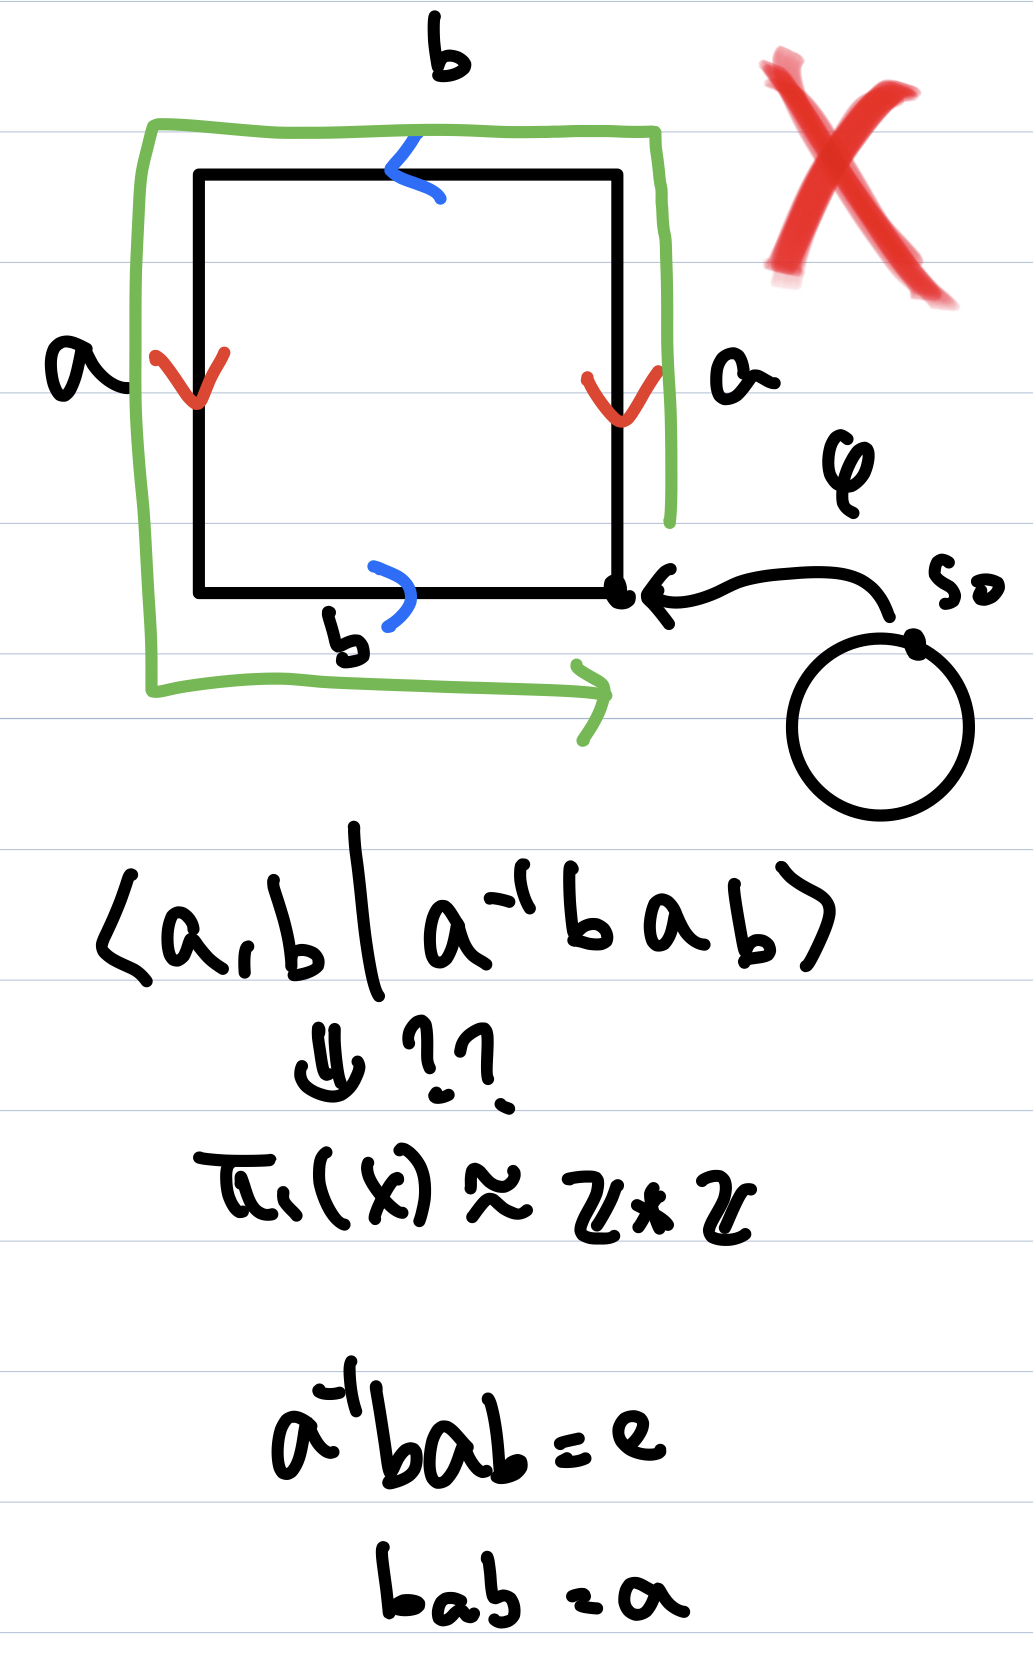
\includegraphics[width=.5\linewidth]{pi_klein.jpeg}
      \caption{Attempt}
    \label{fig:attempt_pi_klein}
  \end{figure}
\end{proof}

\begin{exer}{(Problem 14, Chapter 1.2)}
  Consider the quotient space of a cube $I^3$ obtained by identifying each square face with the opposite square face via the right-handed screw motion consisting of a translation by one unit in the direction perpendicular to the face combined with a one-quarter twist of the face about its center point.
  Show this quotient space $X$ is a cell complex with two 0 cells, four 1 cells, three 2 cells, and one 3 cell.
  Using this structure, show that $\pi_1(X)$ is the quaternion group $\{ \pm 1, \pm i, \pm j, \pm k \}$ of order eight.
\end{exer}

\begin{proof}
  \todo[inline]{
    Tried for 20 minutes.
    I was able to identity 0-cells, 1-cells, 3-cells, but I can't tell what would be 2-cells.
    I think it'll be even harder to figure out the fundamental group.
  }
  \begin{figure}
    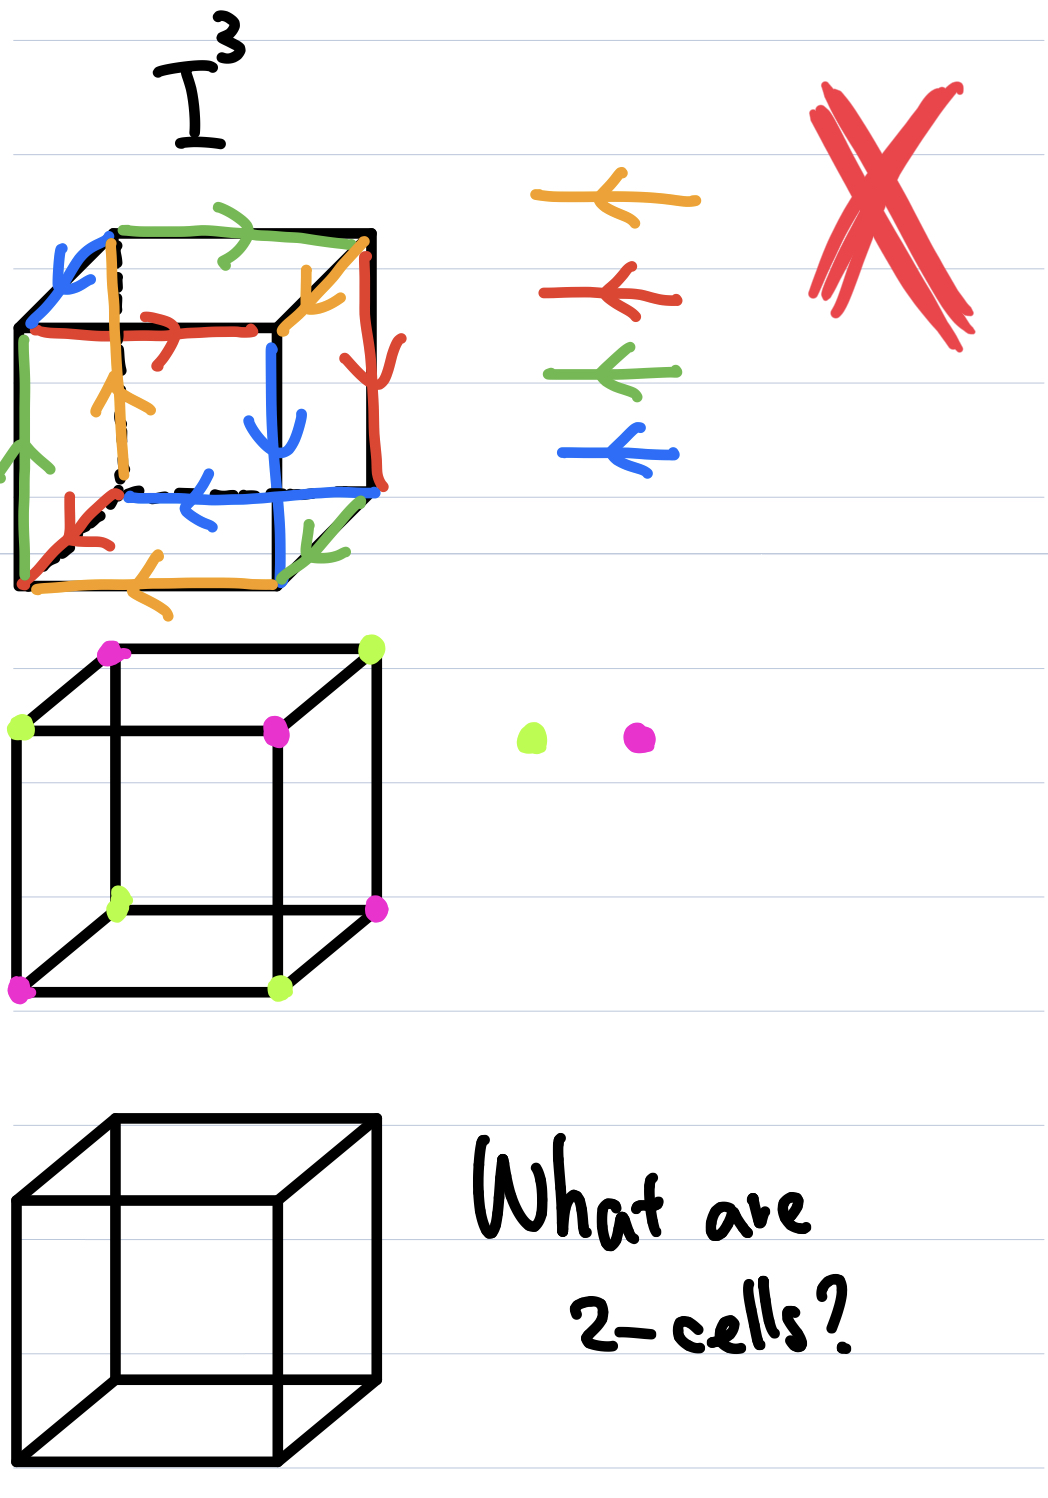
\includegraphics[width=.5\linewidth]{cube_quotient_delete.jpeg}
    \caption{Quotient}
    \label{fig:quotient_delete}
  \end{figure}
\end{proof}

\end{document}


